\setcounter{chapter}{-1}
\chapter{Introduction}
\section{A tinylang program}
\begin{lstlisting}[caption = A semantically and syntactically correct program in \emph{TinyLang}.]
fn Sq(x:float) -> float {
    return x*x;
}
fn XGreaterY(x:float , y:float) −> bool {
    let ans:bool=true ;
    if (y>x) {ans=false ; }
    return ans ;
}
// Same functionality as function above but using less code
fn XGreaterY_2 (x:float , y:float) −> bool {
    return x>y ;
}

fn AverageOfThree (x:float , y:float , z:float ) −> float {
    let total : flaot = x+y+z;
    return total/3;
}

/*
* Same functionality as function above but using less code .
* Note the use o f the brackets in the expression following
* the return statement .
*/

fn AverageOfThree_2 (x:float , y:float , z:float) −> float {
    return (x+y+z)/3 ;
}
//Execution (program entry point) starts at the first  statement
// that is not a function declaration .
let x : float = 2.4 ;
let y : float = Sq(2.5);
let z : float = Sq (x);
print y ; //6.25
print x * z ; //13.824
print XGreaterY (x , 2.3); // true
print XGreaterY 2(Sq(1.5),y); // false
print AverageOfThree (x,y,1.2); //3.28
\end{lstlisting}











\section{Using a tinylang's compiler}
See folder (\emph{binary}) inside project directory.
\begin{itemize}
    \item Place the \verb!tinylang.jar! and \verb!program.tl! in the same directory.
    \begin{figure}[H]
        \centering
        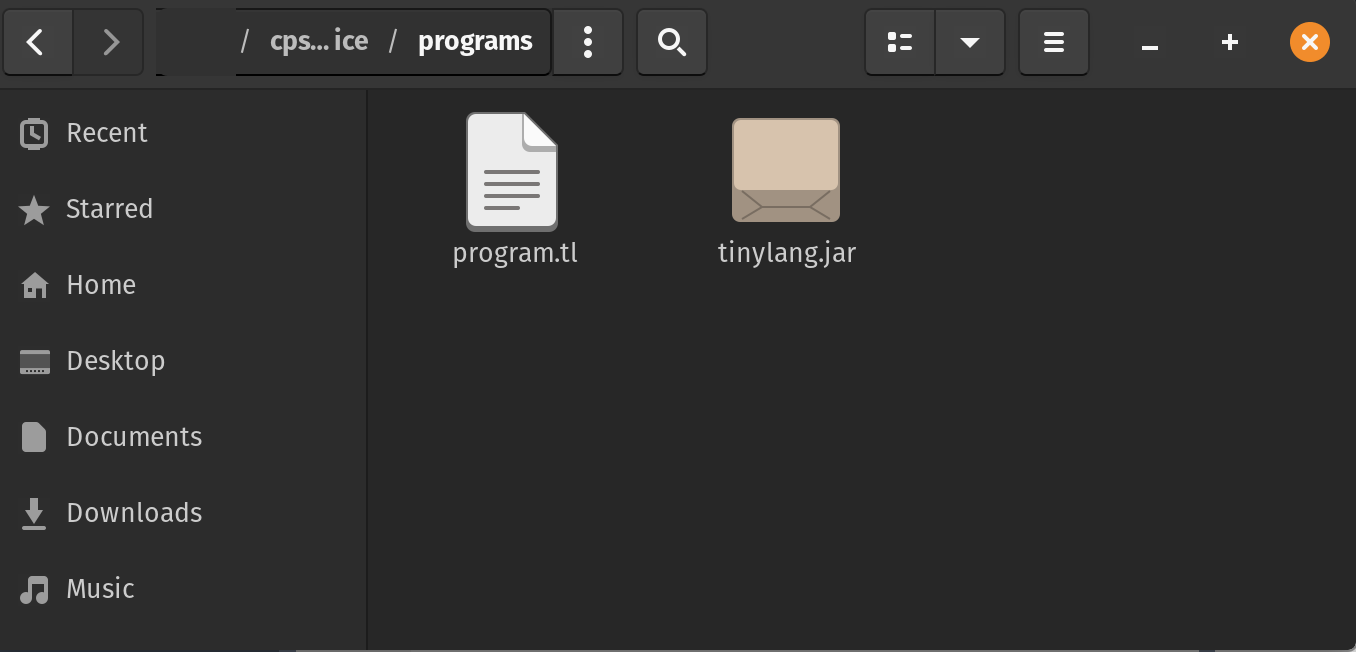
\includegraphics[scale=0.5]{Introduction/images/same_directory.png}
        \caption{Program and compiler binary in same directory.}
        \label{fig:placed in the same directory}
    \end{figure}
    \item Compile \verb!program.tl! using tinylang by running command 
    
    \verb!java -jar tinylang program!
    \item We get a menu:
    \begin{figure}[H]
        \centering
        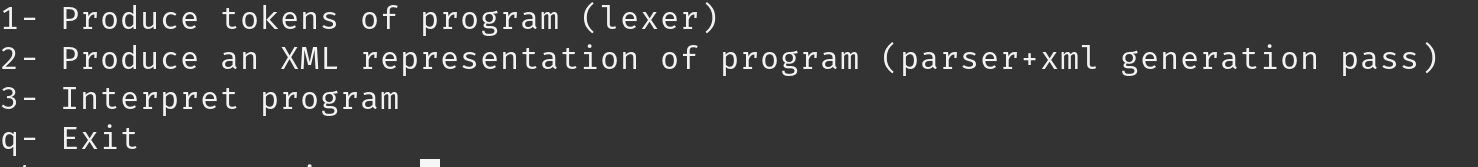
\includegraphics[scale=0.6]{Introduction/images/menu.png}
        \caption{3-option menu}
        \label{fig:3optionmenu}
    \end{figure}

        \begin{figure}[H]
            \centering
           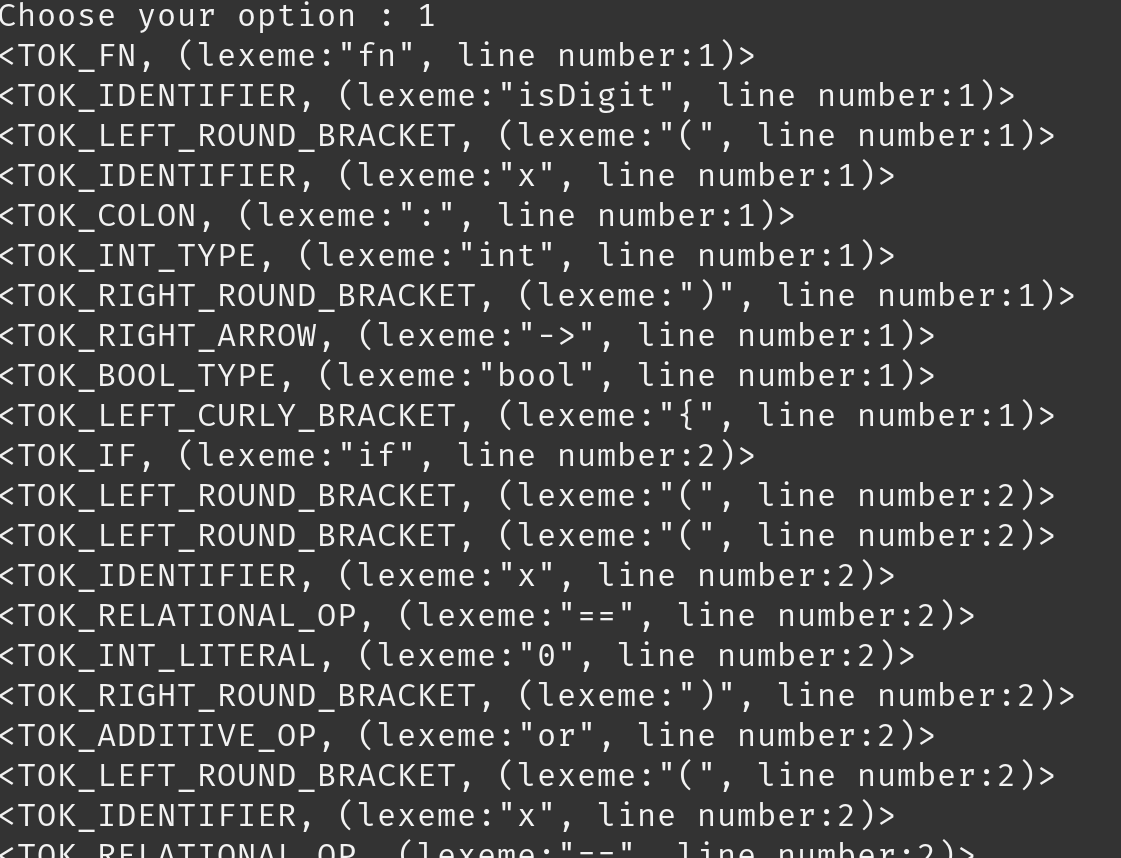
\includegraphics[scale=0.5]{Introduction/images/option1menu.png}
            \caption{Option 1 : Lexer}
            \label{fig:option1 lexer}
        \end{figure}

        \begin{figure}[H]
            \centering
           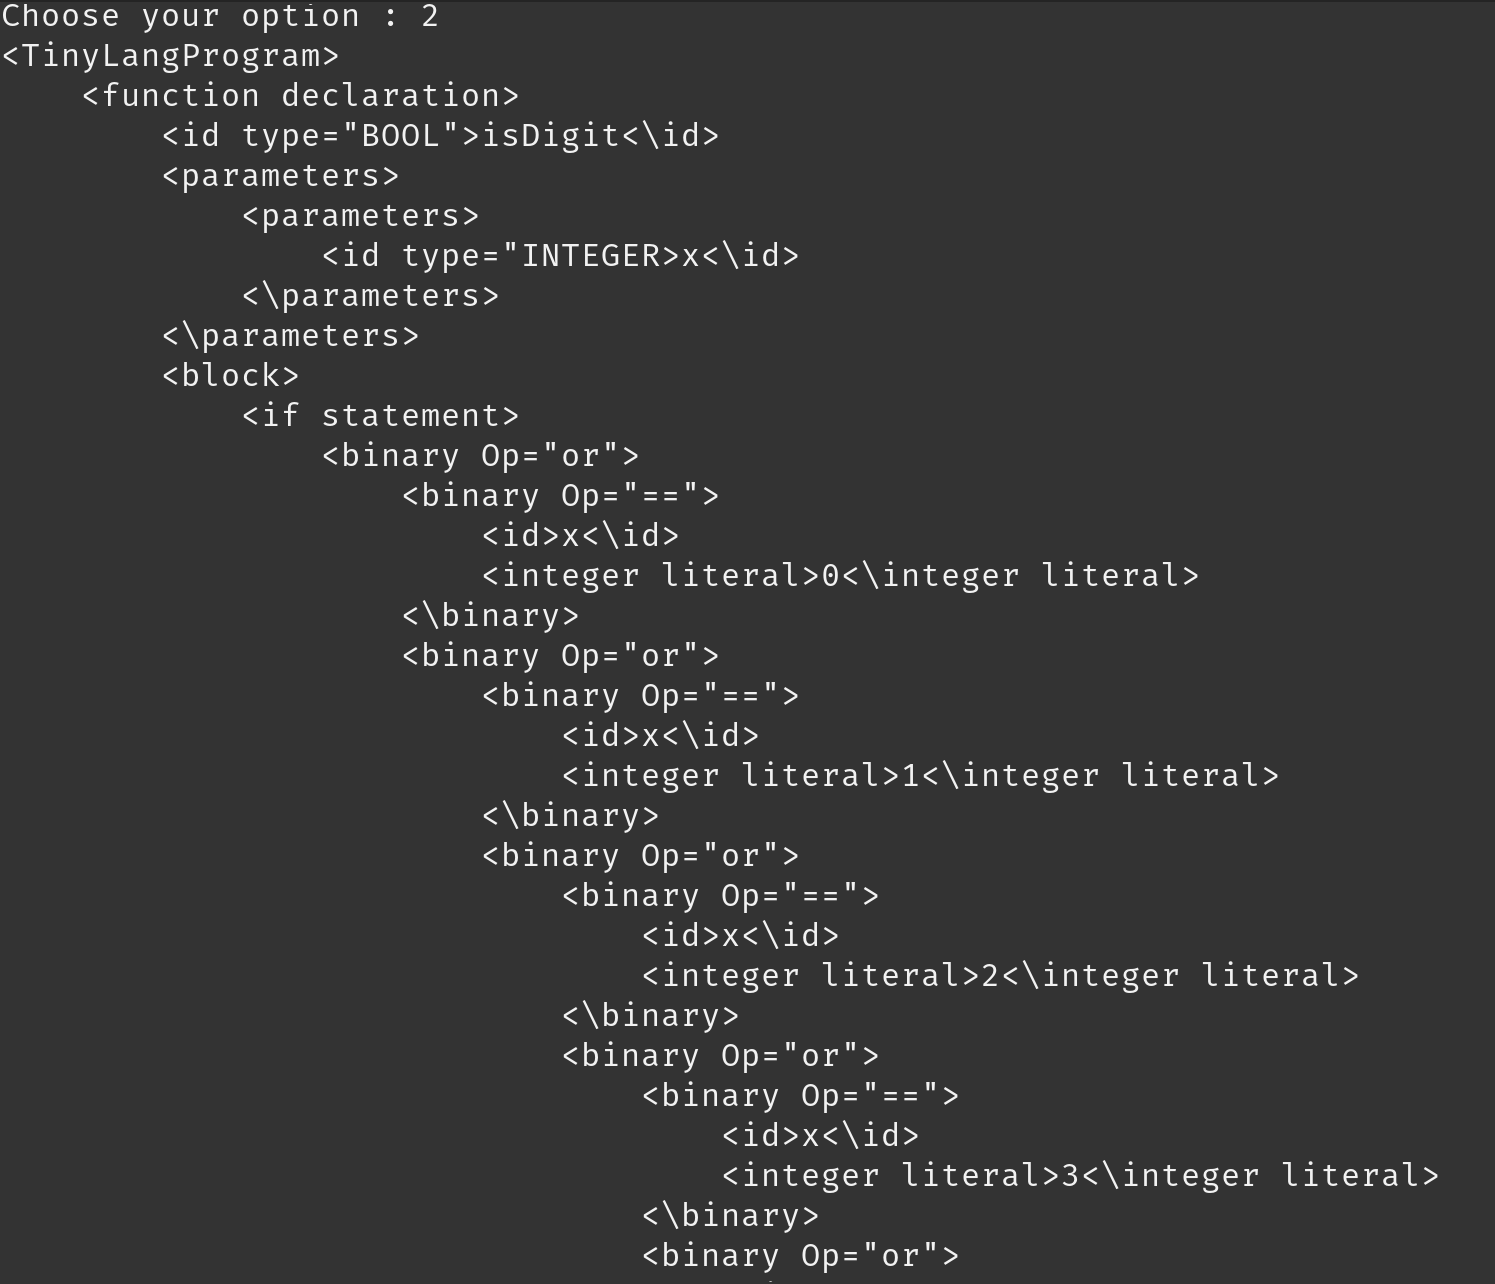
\includegraphics[scale=0.5]{Introduction/images/option2menu.png}
            \caption{Option 2 : XML <-> AST}
            \label{fig:option2 xml}
        \end{figure}    
  
        \begin{figure}[H]
            \centering
           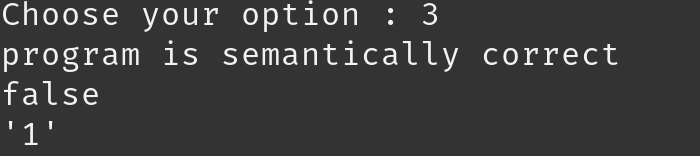
\includegraphics[scale=0.9]{Introduction/images/option3menu.png}
            \caption{Option 3 : confirm that program is semantically correct + interpret}
            \label{fig:opton 3 interpet}
        \end{figure}

    
\end{itemize}




\section{Syntax rules of \emph{TinyLang} in \emph{EBNF}}
\label{sec:ebnf-tinylang-rules}
\begin{lstlisting}[caption = EBNF capturing the Syntax Rules of \emph{TinyLang}.]
<Letter> ::= [A-Za-z]
<Digit> ::= [0-9]
<Printable> ::= [\x20-\x7E]
<Type> ::= 'float'|'int'|'bool'|'çhar'
<BooleanLiteral> ::= 'true' | 'false'
<IntegerLiteral> ::= <Digit>{<Digit>}
<FloatLiteral> ::= <Digit>{<Digit>}'.'<Digit>{<Digit>}
<CharLiteral> ::= '‘' <Printable>'’'
<Literal> ::= <BooleanLiteral> | <IntegerLiteral> | <FloatLiteral> | <CharLiteral>
<Identifier> ::= ('_'|<Letter>){'_'|<Letter>|<Digit>}
<MultiplicativeOp> ::= '*'|'/'|'and'
<AdditiveOp> ::= '+'|'-'|'or'
<RelationOp> ::= '<'|'>'|'=='|'<='|'>='
<ActualParams> ::= <Expression> { ',' <Expression> }
<FunctionCall> ::= <Identifier>'('[<ActualParams>]')'
<SubExpression> ::= '('<Expression')'
<Unary> ::= ('+'|'-'|'not') <Expression>
<Factor> ::= <Literal> | <Identifier> | <FunctionCall> | <SubExpression> | <Unary>
<Term> ::= <Factor> {<MultiplicativeOp> <Factor>}
<SimpleExpr> ::= <Term> {<AdditiveOp> <Term>}
<Expression> ::= <SimpleExpr> {<RelationalOp> <SimpleExpr>}
<Assignment> ::= <Identifier>'='<Expresssion>
<VariableDecl> ::= 'let' <Identifier> ':' <Type> '=' <Expression>
<PrintStatement> ::= 'print' <Expression>
<RtrnStatement> ::= 'return' <Expression>
<IfStatement> ::= 'if' '('<Expression>')' <Block> ['else' <Block>]
<ForStatement> ::= 'for' '('[<VariableDecl>]';'<Expression>';'[<Assignment>]')' <Block>

<WhileStatement> ::= ‘while’ ‘(’ 〈Expression〉 ‘)’ 〈Block〉

<FormalParam> ::= <Identifier> ‘:’ <Type>

<FormalParams> ::= <FormalParam> {','<FormalParam>}

<FunctionDecl> ::= 'fn' <Identifier> '(' [<FormalParams>] ')' '->'<Type><Block>

<Statement> ::= <VariableDecl>';' 
            | <Assignment>';'
            | <PrintStatement>';'
            | <IfStatement>
            | <ForStatement>'
            | <WhileStatement>
            | <RtrnStatement>';'
            | <FunctionDecl>
            | <Block>
<Block> ::= '{' { <Statement> } '}'        
<Program> ::= '{ <Statement> }         
            
\end{lstlisting}

\section{Outline}
\begin{itemize}
    \item tinylang is written in Java and built with the following components:
    \begin{itemize}
    \item \textbf{lexer} which takes a whole program as one string an breaks it down into a sequence tokens.
    \item \textbf{parser} which takes all tokens produced by lexer and produce an abtract syntax tree highlighting the logic of the whole program by parsing the program using the EBNF rules shown above and highlighting syntactical errors in the process.
    \item \textbf{xml generator} produces an indented XML highlighting the structure of the tree (indentation) and all its nodal properties (tags).
    \item \textbf{semantic analyser} used to perform semantic checks such as type checking, checking if a function returns, handling undeclared functions/vars etc.
    \item  \textbf{interpreter } used traverse the program AST and simulates a live execution of the program.
    \end{itemize}
\end{itemize}